\documentclass[iop]{emulateapj}
\usepackage[utf8]{inputenc}

\newcommand{\sick}{\texttt{sick}}
\newcommand{\article}{\textit{Article}}

\usepackage{amsmath}
\usepackage{bm}
\usepackage{natbib}
\usepackage{graphicx}

\begin{document}

\title{\sick, the spectroscopic inference crank}

\author{Andrew R. Casey\altaffilmark{1}}

\altaffiltext{1}{Institute of Astronomy, University of Cambridge, Madingley Road,
Cambdridge, CB3 0HA, United Kingdom; \email{arc@ast.cam.ac.uk}}

\begin{abstract}
In this \article{}  I  introduce \sick{}, the spectroscopic inference crank, an 
open source probabilistic code for inferring astrophysical parameters from 
spectra. \sick{} enables any user to easily construct an approximate 
\textit{generative model} for spectral data, allowing for precise inference for 
a host of astrophysical quantities. Model fluxes (or intensities) are approximated 
by efficient multi-dimensional interpolation of pre-computed spectra. This allows 
any user to capitalise on the plethora of published synthetic and observed spectral 
libraries with minimal effort. Additional phenomena that transform the data 
(e.g., redshift, continuum, smoothing) are incorporated as free parameters. 
Outlier pixels (e.g., cosmic rays or poorly modelled regimes) can be treated with 
a mixture model, and a simplistic noise model is included to account for 
systematically underestimated variance. Combining these phenomena into a 
scalar-justified, quantitative model allows for precise inference with credible 
uncertainties. Commonly employed features are introduced, and the implementation 
details are described. I demonstrate the utility of a generative model approach 
with accurate and precise stellar photospheric measurements from noisy (e.g., 
S/N $\sim{} 7$) high- and low-resolution spectra. \sick{} is very easy to use, 
well-tested, parallelised, and freely available online through GitHub under the 
MIT license. 
\end{abstract}

\section{Introduction}
Most of our understanding of astrophysics has been interpreted from spectra. 
Given how informative spectroscopic data is to our understanding of astrophysics, 
it is not surprising that the last decade has seen a substantial increase of 
publicly accessible spectral data. Large scale surveys have driven this trend, 
each releasing in excess of hundreds of thousands \citep[e.g.,][]{wigglez,boss,
segue,rave,gaia-eso} of spectra. Millions more spectra are expected in the 
coming years \citep[e.g.,][]{lamost,galah}.
 
The spectra are obtained from different astrophysical sources to meet specific 
scientific objectives, and the data vary in wavelength coverage, resolution, and 
noise distributions. For these reasons many collaborations expend significant 
resources to produce bespoke analysis software. Unfortunately this impedes 
scientific reproducibility, as many codes still remain closed-source more than 
a decade after the original article was published. Any comprehensive literature 
comparison subsequently becomes impossible, as systematics can be difficult to 
accurately characterise without in-depth knowledge of the methods or access to 
the software.

Broadly speaking there are three types of methods employed for spectral analysis: 
measuring the strengths of spectral features, pure data-generating models or 
template-matching methods. Approaches that measure spectral features are 
inexpensive, but regularly encounter problems with blended (often hidden) lines 
or continuum placement. As such, some subjective interaction, tuning, or ad-hoc 
`calibration' is almost always required. Data-generating methods compute model 
spectra at run-time, and whilst accurate, can be prohibitively expensive for 
large samples. For template-matching methods, synthetic spectra are only 
generated once to produce a grid of fluxes or intensities for a subset of 
permutations of astrophysical quantities. Although there are differences between 
these methods, the preparatory steps are usually the same. Spectra are placed at 
rest-frame by calculating line-of-sight velocities, typically by 
cross-correlation, before being continuum-normalised to flux intensities. 

Credible uncertainties can be difficult to discern from these approaches. The 
implied assumptions of a $\chi^2$ distribution are often inapplicable, and 
uncertainties in the doppler-shift, smoothing, and normalisation steps are 
almost always ignored. These effects result in ill-characterised uncertainties 
in astrophysical parameters. Alternatively the uncertainties are frequently 
assumed to be approximately the same for all objects.  This is an incorrect 
approach: there are few, if any, examples of homoscedastic datasets in 
astrophysics. The noise properties of each spectrum \textit{are} different, and 
the parameter uncertainties (random and systematic) will differ for every object. 
Consequently the uncertainties in astrophysical parameters by template-matching 
methods are generally found to either be incorrectly assumed, under-estimated, 
or at least ill-characterised. 

In addition to affecting the uncertainties, the effects of redshift, continuum 
normalisation and smoothing \textit{will} systematically bias the reported 
maximum-likelihood parameters. Experienced spectroscopists will frequently 
differ in their decision of continuum placement, even in the most 
straightforward cases (e.g., metal-poor stars). For example, there are a number 
of controversial examples within the literature where the subjective (human) 
decision of continuum placement have significantly altered the scientific 
conclusions \citep[e.g., see][where this issue is discussed in great 
detail]{kerzendorf}. The implications of these phenomena \textit{must} be 
considered if we are to understand subtle astrophysical processes. Spectroscopy 
requires objectivity: one should endeavour to incorporate these phenomena as 
free parameters into a generative model and infer them simultaneously with the 
astrophysical parameters.

In this \article{} I present \sick{}: a well-tested, MIT-licensed probabilistic 
software package for inference from spectroscopic data. \sick{} employs an 
approximation to data-generating models. Instead of attempting to model all 
kinds of expensive astrophysical processes (e.g., stars, supernova, 
and any other interesting astrophysical processes) at run-time, it performs 
efficient multi-dimensional interpolation of model spectra from pre-computed 
grids and includes contributory phenomena (e.g., continuum, redshift) as free
parameters within an objective scalar-justified model. This approach is suitable 
for a plethora of different astrophysical 
processes, allowing any user to easily specify a model using existing published 
spectral grids, and infer astrophysical properties from their data. Aspects of 
the probabilistic model are described in Section \ref{sec:model}. A number of 
examples are included in Sections \ref{sec:inference-test} and \ref{sec:examples}, 
where I present accurate and precise objective photospheric measurements using 
noisy spectra. I conclude in Section \ref{sec:conclusions} with references to 
the online documentation and applicability of the software.

\section{The Generative Model}
\label{sec:model}

The primary advantage of \sick{} is the simultaneous inference of both 
astrophysical and other pertinent parameters that can alter the spectra. The 
generative model described here is agnostic as to \textit{what} the 
astrophysical parameters actually describe. Typical examples might be properties 
of supernova (e.g., explosion energies and luminosities), galaxy characteristics 
from integrated light, or mean plasma properties of a stellar photosphere. There 
are a plethora of spectral libraries (observed and synthetic) published for these 
types of applications \citep[e.g.,][]{snid,pegase,phoenix,pollux}. All of these 
models are fully-\sick{} compatible. However given the research background of 
the author, I will introduce the probabilistic model by focussing on stellar 
photospheric inferences.

The first step of the (approximate\footnote{The term approximate is used because 
model spectra are interpolated.}) generative model is to interpolate a model 
spectrum. \sick{} employs the Quickhull algorithm \citep{quickhull} to linearly 
interpolate in multiple dimensions. Irregularly-spaced grids are perfectly 
acceptable; Quickhull does not require the grid to be rectangular or 
regularly-spaced points. Large grids of model spectra are cached for 
computational efficiency, allowing for the total size of the model grid to far 
exceed the available random access memory.\footnote{In practice this is performed 
by efficient memory-mapping.} I introduce an interpolation function $S(\bm{\psi})$ 
that produces a model spectrum with $J$ points $\{\lambda_j,I_j\}_{0}^{J}$ at 
any evaluable point $\bm{\psi} \equiv (T_{\rm eff},\log{g},{\rm [M/H]},[\alpha/{\rm Fe}])$ 
within the grid boundaries.

\begin{equation}
S(\bm{\psi}) \rightarrow \{\lambda_j,I_j\}
\end{equation}

The model spectrum $S(\bm{\psi})$ should always be of higher spectral resolution 
than the data. Therefore it is necessary to smooth (or broaden) $\{\lambda_j,I_j\}$ 
with a Gaussian filter of standard deviation $\sigma_{s}$ such that it matches 
the spectral resolution of the data. For some applications it is tempting to 
perform this step \textit{a priori} from the instrument spectral resolution. 
However it is not necessarily true that the quoted instrumental resolution will 
perfectly match the data. In truth the data have a \textit{distribution} of 
spectral resolutions. Even if the spectral resolution is accurately known with 
low variance, fixing this value will result in under-estimated uncertainties 
$\sigma(\bm{\psi})$ and likely bias the posterior distribution distributions for 
$\bm{\psi}$. Employing the free parameter $\sigma_{s}$ allows for the 
identification of additional instrumental or atmospheric broadening. For stellar 
applications, the free parameter $\sigma_{s}$ also aids in the identification of 
unresolved binary companions.

The doppler shift of the source is treated by transforming the model spectrum 
(in uniformly sampled $\log\lambda$ space). \sick{} solves for redshift $z$ 
(Equation \ref{eq:redshift}), and returns posterior distributions in the user's 
preferred units (e.g., km s$^{-1}$).

\begin{equation}
\label{eq:redshift}
\lambda_{s} = \lambda_{j}(1 + z)
\end{equation}

After the model spectrum is smoothed and doppler shifted, model intensities are 
required at the wavelengths $\lambda_i$ of the observed pixels. The complete 
function to yield model intensities $M_i$ at wavelengths $\lambda_i$ is therefore 
a function of the parameters of interest $\bm{\psi}$, redshift $z$, smoothing 
kernel $\sigma_{s}$, and the wavelengths of the observed pixels $\lambda_i$:

\begin{equation}
 M_{i} \equiv S\left(\bm{\psi},z,\sigma_{s},\lambda_i\right)
\end{equation}

In principle there is no reason to believe that the doppler-shifted, smoothed 
model intensities $M_i$ should match the data at all. The counts and shape of 
observed fluxes are a function of source magnitude, exposure time, instrument 
sensitivities, atmospheric conditions, and a host of unaddressed effects. In 
contrast the model spectra are calculated either as intensities (e.g., $I_j$) 
or fluxes calibrated to an empirical system. Even for the true values of 
$\bm{\psi}$, a function is required to normalise\footnote{The normalisation 
process is frequently abused by stellar spectroscopists in the literature. 
Wherever possible, data should not be transformed. One should seek to fit a 
model to the data, not the other way around.} the model to the data. As such I 
transform the \textit{model} intensities by some function $C$ to fit the data. 
Although the function $C$ incorporates a number of effects (e.g., source 
blackbody temperature, dust, instrument sensitivities), they are phenomena that 
typically cannot be separated without additional information, and here I only 
care about their combined effect. I only wish to ensure that the overall shape 
of the data are accounted for, which is usually achievable with a low-order 
polynomial

\begin{equation}
C_i = c_{0}\lambda_{i}^{m-1} + c_{1}\lambda_{i}^{m-2} + \dots + c_{m}
\end{equation}

\noindent{}with $m$ free coefficients $c_{0\dots{}m}$, where $m$ is specified by 
the user. Other continuum functions are available in \sick{}, and the user is 
encouraged to experiment for a specific problem. This allows us to express the 
\textit{expected flux} $E_i$ at a given observed pixel with wavelength $\lambda_i$ as:

\begin{equation}
E_i = S_{i}\times{}C_i
\end{equation}

In many astrophysical cases the flux uncertainties $\sigma_{i}$ for a given pixel 
are not well-characterised. This is often due to unpropagated uncertainties during 
data reduction. Since the observed flux counts are expected to be Poisson-distributed, 
in many astrophysical scenarios the pixel flux uncertainty can be made estimated 
as $\sigma_i \sim 1/\sqrt{F_{i}}$. Knowing that this approximation may underestimate 
the noise, I include an additional parameter to account for the possibility that 
the variance in all pixels is underestimated by some fractional amount $f$ 
(Equation \ref{eq:noise-model}). While this crude noise model is probably 
unrepresentative of the data in a large number of cases, including \textit{any} 
noise model is preferable to none.

\begin{equation}
s_{i}^2 = \sigma_{i}^2 + f^{2}E_{i}^2
\label{eq:noise-model}
\end{equation}

We now have a \textit{generative model} for the data. The frequency (or 
probability) distribution ${p\left(F_i|\lambda_i,\sigma_i,\bm{\psi},z,\sigma_s,\{c\}_{0}^{m}\right)}$ 
for the observed data $F_i$ is given by

\begin{equation}
p\left(F_i|\lambda_i,\sigma_{i},\bm{\psi},z,\sigma_{s},\{c\}_{0}^{m},f\right) = 
 \frac{1}{\sqrt{2\pi{}s_{i}^2}}\exp{\left(-\frac{\left[F_i - E_i\right]^2}{2s_{i}^2}\right)}
 \label{eq:p_model}
\end{equation}

\noindent{}and with the implied assumption that the data are independently drawn,
the likelihood $\mathcal{L}$ is calculable by the product of individual probabilities:

\begin{equation}
\mathcal{L} = \prod_{i=1}^{N}\,p\left(F_i|\lambda_i,\sigma_{i},\bm{\psi},z,\sigma_{s},\{c\}_{0}^{m},f\right)
\end{equation}

From the original astrophysical parameters $\bm{\psi}$ that I care about, I now 
have an additional $3 + m$ parameters to consider. The situation seemingly becomes 
more complex when separately observed channels are considered. Many spectrographs 
provide small portions of spectra (a channel, also colloquially expressed as beams 
or apertures) separated by some large gap. The data for each channel are usually 
captured by different CCDs and are therefore reduced separately. 

The instrumental parameters $\sigma_{s}$, $\{c_k\}_{k=0}^{m}$, and $f$ are likely 
to be different for each channel. Although redshift $z$ is an astrophysical effect 
and should not differ between channels, this may not be true if each channel has 
been wavelength-calibrated differently. It is therefore prudent to introduce 
separate parameters $z$, $\sigma_{s}$, $\{c_k\}_{k=0}^{m}$, $f$ for \textit{each} 
of the $N_{chan}$ observed channels. This scales the total dimensionality of the 
model as $3\times{}N_{chan} + \sum_{k=0}^{N_{chan}}m_{k}$ in addition to $\bm{\psi}$. 
The inclusion of all of these parameters is not mandatory: each \sick{} model can 
be adjusted to include or ignore any combination of phenomena. 

Finally, I consider the handling of outliers in the data. These may be in the form 
of cosmic ray spikes, improper calibration of the data, telluric features, or simply 
poorly modelled spectral regions. Treatment of these artefacts is achieved using a 
Gaussian mixture model: a combination of two models. In a mixture model, the data 
are fit by the sum of amplitudes ($1 - P_o$ and $P_o$, respectively) of two 
distributions: the expected fluxes $E_i$, and a normal distribution centered along 
the continuum function $C_i$ with variance $s_{i}^2 + V_{o}$. This requires the 
inclusion of two  additional parameters: $P_o$ and $V_o$. The prior 
distribution function $p\left(V_o\right)$ requires $V_{o}$ to always be positive 
(Equation \ref{eq:default_priors}), and as such the outlier distribution will 
\textit{always} have a larger variance. Distributions of smaller variance are more 
informative, so conceptually a fit to the expected fluxes $E_{i}$ is generally 
preferred wherever possible. For brevity I define $\bm{\kappa} \equiv (\bm{\psi},\{z,\sigma_s,\{c_k\}_{k=0}^{m},f\}_{0}^{N_{c}})$, and the likelihood for the mixture model is given by
 
 \begin{equation}
\mathcal{L} = \prod_{i=1}^{N}\,\left[\left(1 - P_{o}\right)\times{}p_{model}\left(F_i|\lambda_i,\sigma_{i},\bm{\kappa}\right) + P_{o}\times{}p_{outlier}\left(F_i|\lambda_i,\sigma_i,\bm{\kappa},V_{o},P_o\right)\right]
\end{equation}
 
\noindent{}where $p_{model}$ refers to $p$ in Equation \ref{eq:p_model} and 

\begin{equation}
p_{outlier}\left(F_i|\lambda_i,\sigma_i,\bm{\kappa},V_{o},P_o\right) = \frac{1}{\sqrt{2\pi\left(s_{i}^2 + V_{o}^2\right)}} \exp\left(-\frac{[F_i - C_i]^2}{2\left[s_{i}^2 + V_{o}^2\right]}\right)
\end{equation}

\noindent{}such that the likelihood $\mathcal{L}$ becomes:

\begin{equation}
\mathcal{L} = \prod_{i=1}^{N} \left[ \frac{1-P_o}{\sqrt{2\pi{}s_{i}^2}}\,\exp\,\left(-\frac{[F_i - E_i]^2}{2s_{i}^{2}}\right) + \frac{P_o}{\sqrt{2\pi\left[s_{i}^2 + V_o\right]}}\,\exp\,\left(-\frac{[F_i - C_i]^2}{2\left[s_{i}^{2} + V_o\right]}\right)\right]
\label{eq:full_likelihood}
\end{equation}

I define the full parameter space with $\bm{\theta} \equiv \left(\bm{\psi},\{z,\sigma_s,\{c_{b_k}\}_{k=0}^{m},f\}_{b=0}^{N_{c}},V_o,P_o\right)$. From Bayes theorem the posterior probability 
distribution for $\bm{\theta}$ (up to a constant) is given by
\begin{eqnarray}
\mathcal{P} & \propto & likelihood \times prior \nonumber \\
p(\bm{\theta}|\{F_i\}_{i=1}^{N}) & \propto & p(\{F_i\}_{i=1}^{N}|\bm{\theta})\,\times\,p(\bm{\theta})
\label{eq:probability}
\end{eqnarray}

\noindent{}where $p(\bm{\theta}|\{F_i\}_{i=1}^{N})$ is the probability $\mathcal{P}$ 
of $\bm{\theta}$ given the data (and given the model: e.g., see Section \ref{sec:sun}), 
$p(\{F_i\}_{i=1}^{N}|\bm{\theta})$ is our previously defined likelihood function 
$\mathcal{L}$ (Equation \ref{eq:full_likelihood}), and $p(\bm{\theta})$ is the prior 
probability distribution. Priors are discussed in more detail in Section \ref{sec:mcmc}. 

% Log probability, expand function
%\begin{eqnarray}
%\log({\mathcal{P}}) & \propto & \log{likelihood} + \log{prior} \nonumber \\
%\log(\mathcal{P}) & \propto & \prod_{i=1}^{N} \left[ \frac{1-P_b}{\sqrt{2\pi\sigma_{i}^2}}\,\exp\,\left(-\frac{[F_i - E_i]^2}{2\sigma_{i}^{2}}\right) + \frac{P_b}{\sqrt{2\pi\left[\sigma_i^2 + V_o\right]}}\,\exp\,\left(-\frac{[F_i - C_i]^2}{2\left[\sigma_i^{2} + V_o\right]}\right)\right] \nonumber \\
%& & \dots +  \ln(p(\bm{\theta}))
%\end{eqnarray}

With all of the combined effects there are 16 free parameters including $\bm{\psi}$, 
the astrophysical quantities of interest. For the examples presented in Section 
\ref{sec:examples}, this requires interpolation between $9.2 \times 10^{10}$ pixels in four 
dimensions. While the description might appear daunting, the problem is tractable, 
numerically efficient, and easy to configure. By default \sick{} numerically solves 
this problem in three sequential steps, which are described in the following 
sections: scattering, optimisation, and Monte-Carlo Markov Chain (MCMC) sampling.


\subsection{Initial Scattering}
\label{sec:scattering}

We seek to maximise $\mathcal{P}$ (or in practice, $\log\mathcal{P}$) and calculate
the posterior probability distributions for $\bm{\theta}$ given the data. In the 
first step I calculate the log-probability $\log{(\mathcal{P})}$ for $N_{sample}$ 
randomly drawn points from all over the astrophysical parameter space $\bm{\psi}$. 
Since \sick{} allows for arbitrarily large parameter spaces in $N_{D}$ dimensions, 
initially sampling the parameter space $N_{sample}$ times provides a coarse 
landscape of probability. If the probability distribution function were smoothly 
distributed across all $\bm{\psi}$, or the optimisation step was sufficiently 
robust for all potential applications, then in principle \textit{any} single 
point would be an adequate starting guess. However there is no way of knowing 
\textit{a priori} how smooth the posterior distribution will be for a given problem. 

The $N_{samples}$ points are uniformly drawn in $\bm{\psi}$ by default, unless 
priors are specified (see Section \ref{sec:mcmc}). A model spectrum $S(\bm{\psi})$ 
is interpolated for each point, which is used to estimate the redshift and continuum 
parameters. After smoothing the model fluxes $I_j$ by $\sigma_s$ (as drawn from an 
explicit prior, or estimated by $\left|\mathcal{N}\left(0, 1\right)\right|$) the 
smoothed spectrum is cross-correlated with the data to yield a redshift estimate. 
Continuum parameters $\{c_k\}_{k=0}^{m}$ are similarly estimated by fitting a 
function (a polynomial in this case) to the data divided by the smoothed flux at 
each $\lambda_i$. Estimating continuum and redshift provides us with a reasonable 
guess of the probability for any randomly scattered point $\bm{\psi_i}$. If outlier 
modelling is included in the model then $P_o$ is distributed as 
$\mathcal{U}\left(0, 1\right)$ by default, and $V_o$ is estimated by 
$\mathcal{N}\left(\widetilde{F_i}, \frac{1}{2}\widetilde{F_i}\right)$. This procedure 
is \textit{only} employed for the initial random scattering stage: it is 
\textit{not} applicable for the MCMC phase. 

\subsection{Optimisation}
\label{sec:optimise}

After the random scattering step, the most probable $\bm{\theta}$ point is used 
as an initial guess for numerical optimisation. A number of suitable minimisation 
algorithms are available in \sick{} through the SciPy \citep{scipy} optimization 
module. The \citet{nelder-mead} algorithm is employed by default.
Unlike other optimisation techniques, the Nelder-Mead algorithm 
does not approximate first- or second-order derivatives, and can consequently be 
less efficient than other approaches. However it is robust in high-dimensional 
space, even in the presence of substantial noise, and has been successfully 
employed in a wide range of engineering and scientific problems. The reader is 
encouraged to experiment with other optimisation approaches if the Nelder-Mead 
algorithm proves unsuitable or takes an untenable amount of time. Since these 
optimisation algorithms are minimisation techniques and I seek to maximise the 
log-probability $\log{\left(\mathcal{P}\right)}$, I numerically optimise the 
parameters $\bm{\theta}$ by minimising the negative log-probability 
$-\log{\left(\mathcal{P}\right)}$.

\subsection{Monte-Carlo Markov Chain Sampling}
\label{sec:mcmc}

The random scattering and numerical optimisation steps efficiently provide an 
accurate estimate of the optimal parameters $\bm{\theta_{opt}}$. Once the optimisation
 step is complete, \sick{} employs the affine-invariant ensemble sampler proposed 
 by \citet{goodman;weare}, and implemented by \citet{emcee}. The Metropolis-Hastings 
 MCMC algorithm is employed by default. \sick{} allows for the model settings to 
 be specified in a human-readable \textsc{yaml}- or \textsc{json}-formatted 
 configuration file\footnote{The reader is referred to the online documentation 
 for an example.}, where the number of Goodman \& Weare walkers can be specified, 
 as well as the number of samples to perform. When the optimisation step is used, 
 the initial points are taken from a small multi-dimensional ball around the 
 optimised parameters $\bm{\theta_{opt}}$. If the optimisation step is not 
 performed, initial values for the MCMC walkers are drawn in the same way as 
 described for the scattering process. 

Priors represent our initial knowledge about a particular parameter before 
looking at the data, and are necessary for any Bayesian analysis. A number of 
different prior distributions can be specified by the user in the \sick{} model 
configuration file. When no prior is explicitly specified, the following 
uninformative prior distributions are assumed (for all channels, where appropriate):

\begin{eqnarray}
p\left(\bm{\psi}_{dim}\right) &=& \mathcal{U}\left(\min\left[\bm{\psi}_{dim}\right], \max\left[\bm{\psi}_{dim}\right]\right) \\
p\left(P_o\right) &=& \mathcal{U}\left(0, 1\right) \\
p\left(\log{f}\right) &=& \mathcal{U}\left(-10, 1\right) \\
p\left(V_o,\sigma_s\right) &=& \left\{
\begin{array}{c l}      
    1\,, &\mbox{for values greater than zero}\\
    0\,, &\mbox{otherwise}
\end{array}\right. \\
p\left(z,\{c_k\}_{k=0}^{m}\right) &=& 1 \\
\label{eq:default_priors}
\end{eqnarray} 

A consequence of allowing irregular model grids is that occasionally a model 
spectrum cannot be interpolated for some values of $\bm{\psi}$, even if they 
fall within $\left(\min\left[\bm{\psi}\right], \max\left[\bm{\psi}\right]\right)$. 
In these cases $p\left(\bm{\psi}\right) = 0$ and thus $\log\left(\mathcal{P}\right) = -\infty$.

Quantitatively ensuring numerical convergence for MCMC analyses remains an 
unsolved problem. There are a number of excellent resources on MCMC sampling 
which outline this issue in greater detail. The mean acceptance fraction, 
auto-correlation times, and values of the parameter chains themselves all 
provide reasonable proxy indicators of convergence. The user is encouraged to 
inspect these metrics and devise some heuristic for when convergence has 
unambiguously been achieved. The final state of every MCMC analysis is 
automatically saved by \sick{}, allowing users to resume their analysis from 
the most recent state if they believe the system has not converged.


\subsection{Self-consistent inference test}
\label{sec:inference-test}

As an initial test of the probabilistic framework I have interpolated a 
noise-free synthetic spectrum which will act as a faux observation. A single 
channel from the AMBRE synthetic library \citep{ambre} has been employed. These 
spectral channels range from 475\,nm to 685\,nm and were specifically calculated 
by the AMBRE group for the Gaia-ESO Survey \citep{gaia-eso}. I have applied a number of transformations to the 
interpolated spectrum: a second-order polynomial enters multiplicatively to 
represent the continuum, the spectrum is redshifted, and fluxes are convolved 
to a spectral resolution of $\mathcal{R} \sim 10000$. The faux data are resampled 
to a uniform spacing of $\sim{}0.08$\,nm, effectively discarding $99.5\%$ of 
the original pixels, which were sampled at $\sim4\times10^{-4}$\,nm. White noise  
has been added to replicate a S/N ratio of $\sim 7$ pixel$^{-1}$. I also assumed 
that the observed variance is systematically underestimated by 10 per cent: 
conceptually the faux data is $\sim{}$10 per cent noisier than what an observer 
would estimate from the flux counts. 


\begin{figure*}
\label{fig:chains}
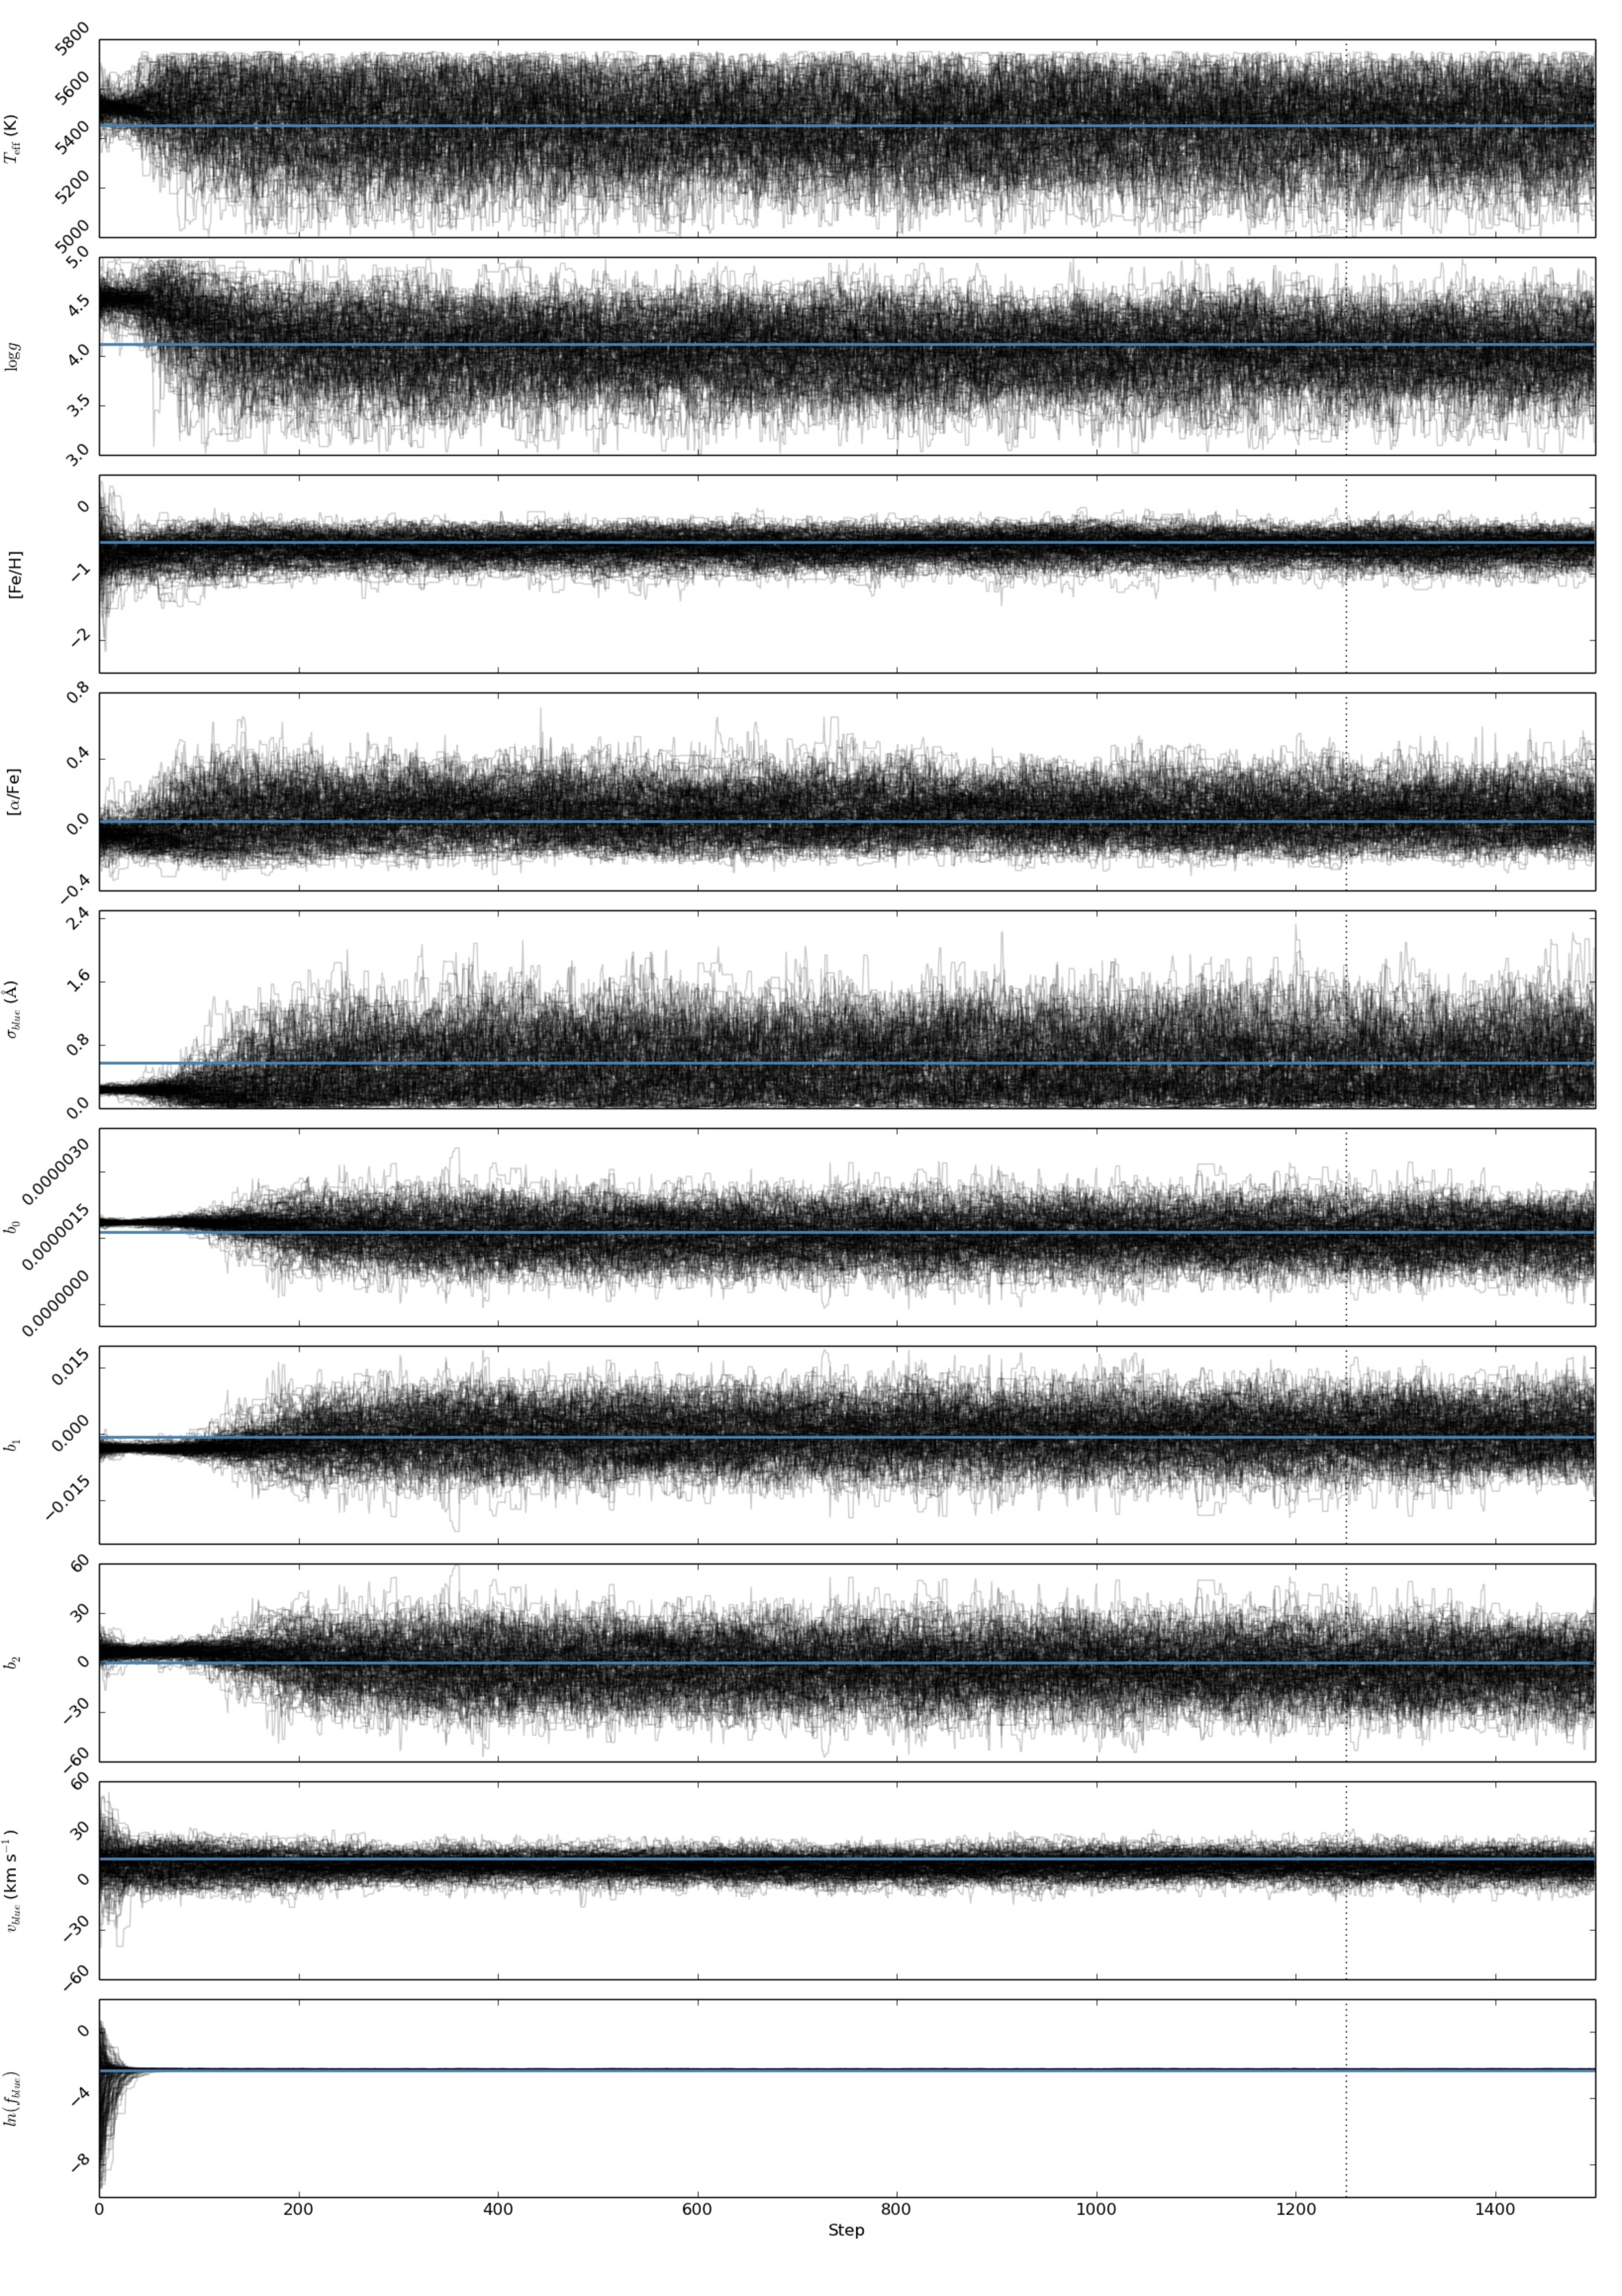
\includegraphics[height=\textheight]{chains.pdf}
\caption{Points sampled by the 200 walkers at each step during the self-consistent 
inference test. The true values are marked in blue. The first 1250 steps are 
discarded as the burn-in period.}
\end{figure*}

\begin{figure*}
\label{fig:corner-inference}
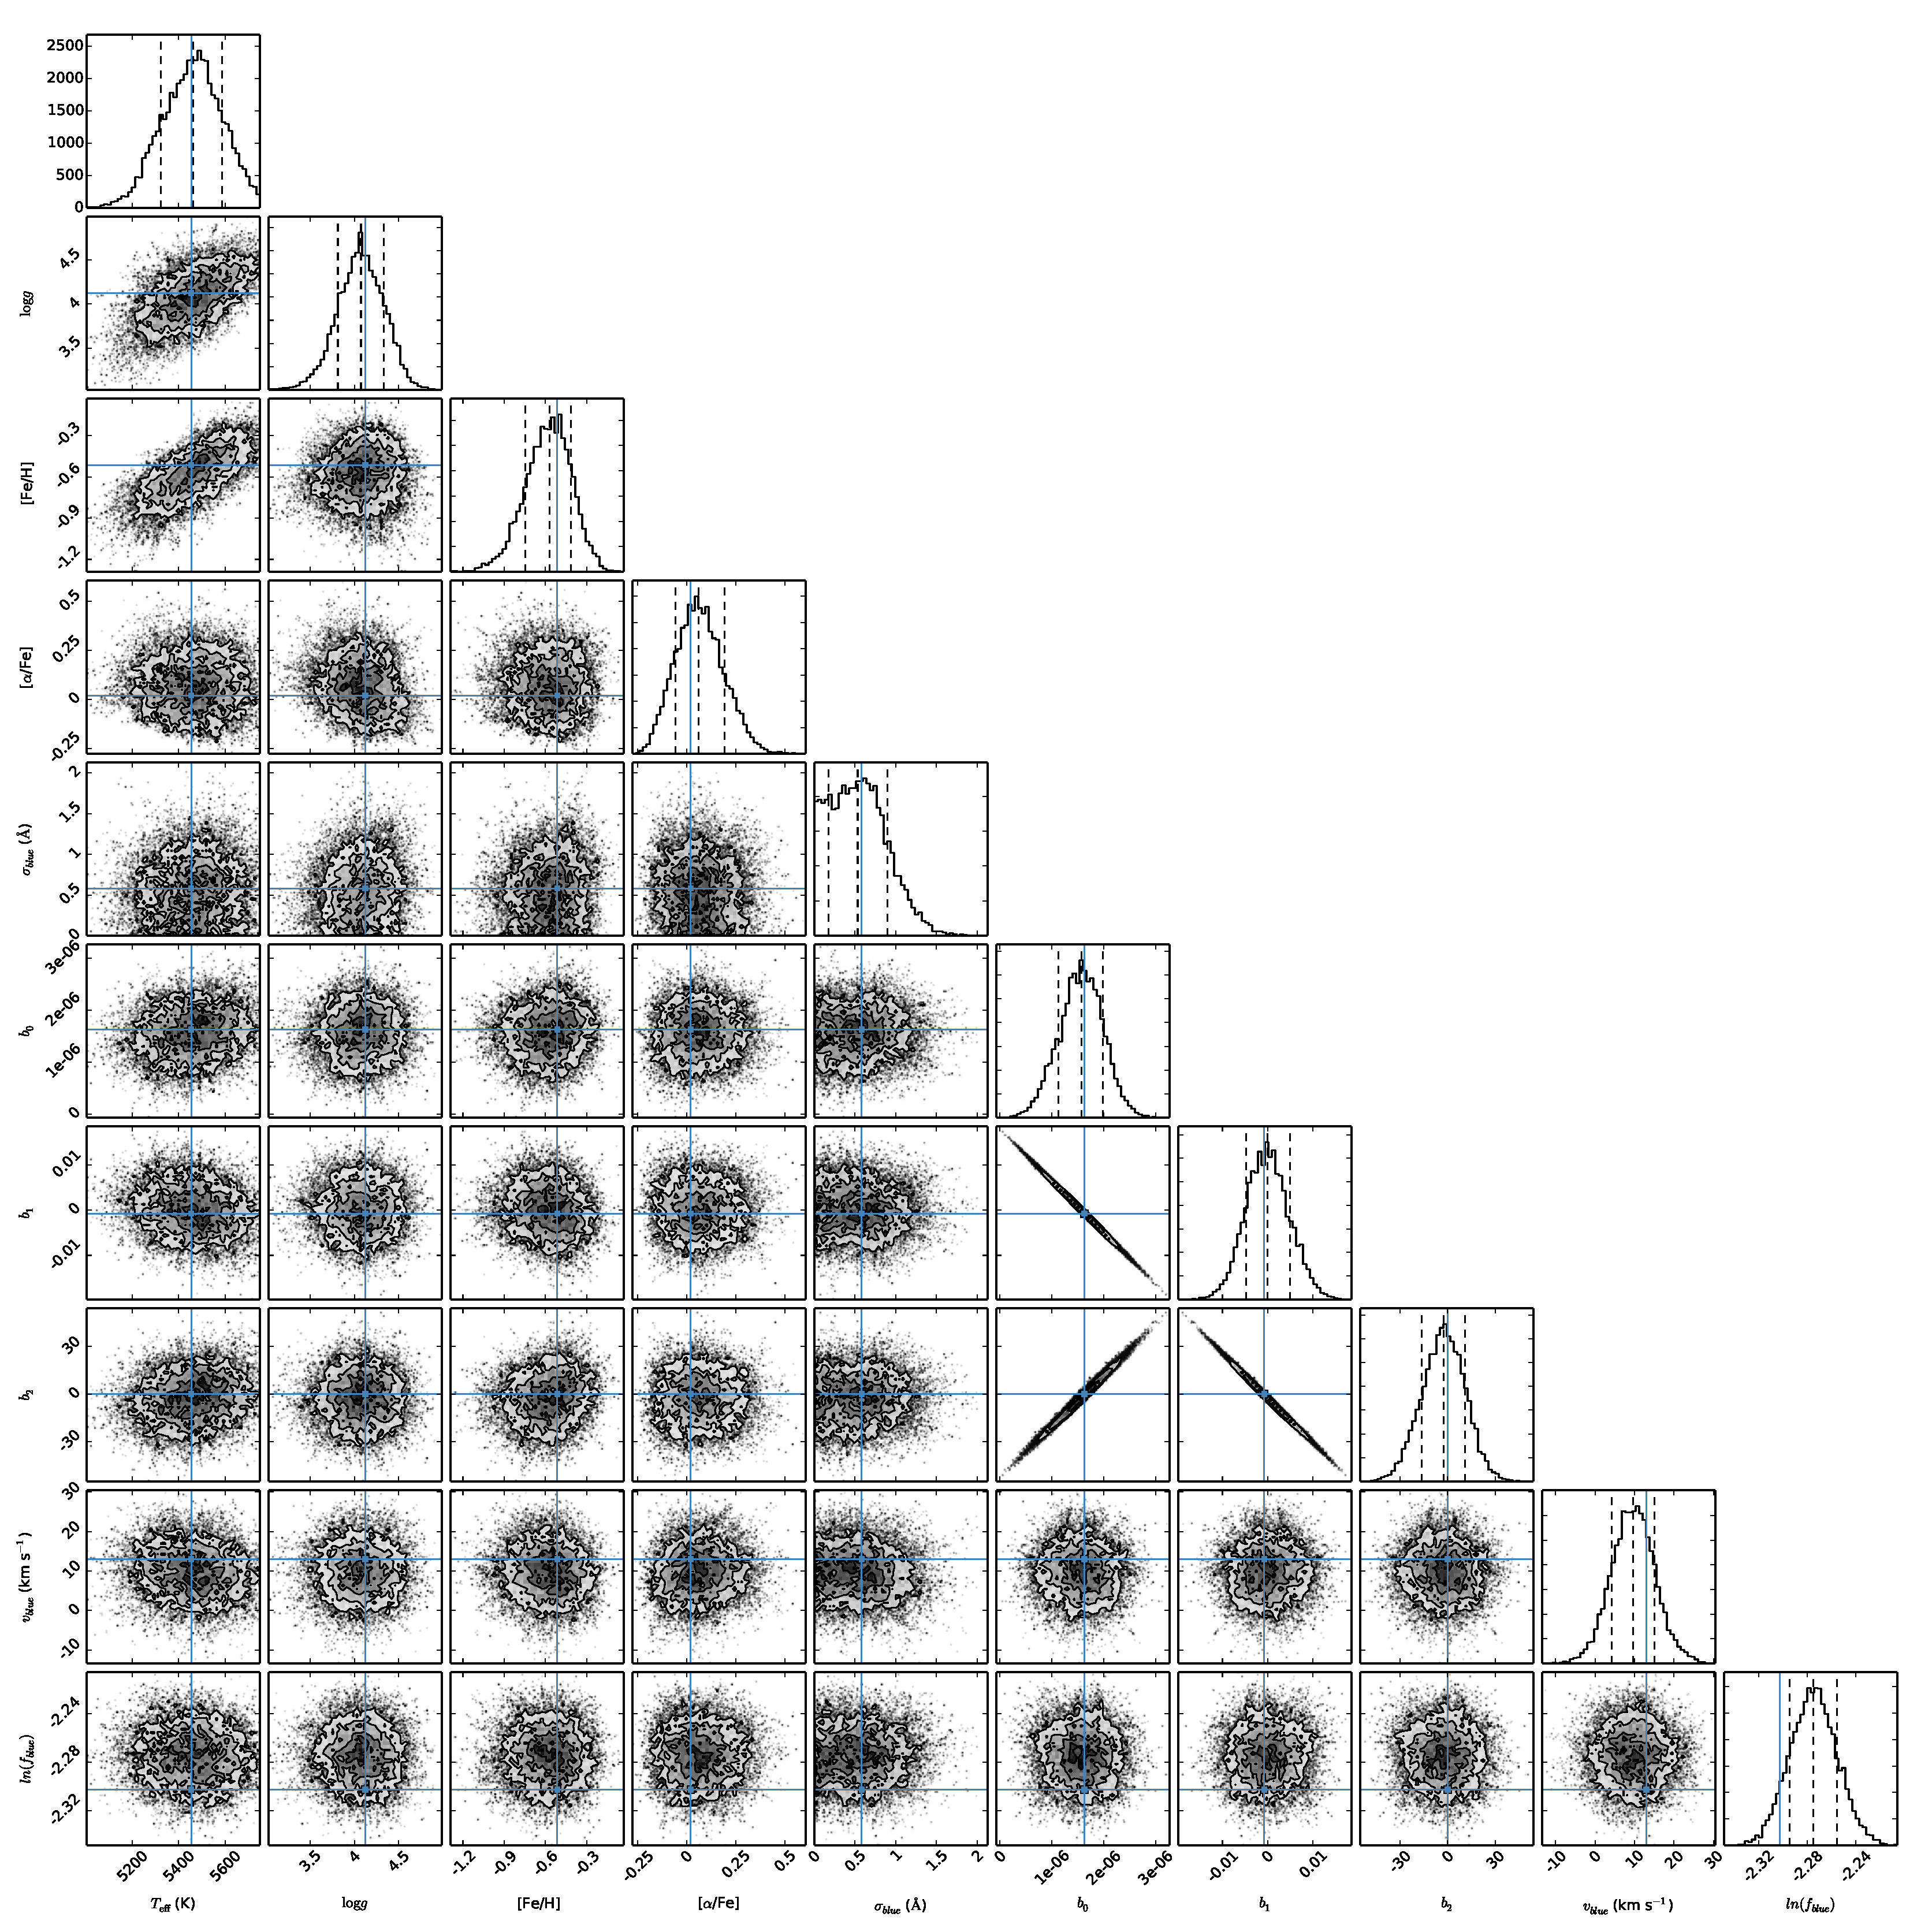
\includegraphics[width=\textwidth,height=\textwidth]{corner.pdf}
\caption{Marginalised posterior distributions for all parameters $\bm{\theta}$ 
from a faux observation with spectral resolution $\mathcal{R} \sim 10,000$ and 
S/N ratio $\sim{}7$\,pixel$^{-1}$. True values are marked in blue. This figure 
demonstrates that precise inference of stellar parameters can be made with 
high-resolution spectra, even in the presence of substantial noise.}
\end{figure*}

\begin{table*}
\center
\caption{True and inferred model parameters for the self-consistent inference test}
\label{tab:inference-test}
\begin{tabular}{llrr}
\hline
\hline
Parameter & Description & Truth & Inferred \\
\hline
$T_{\rm eff}$ & Effective photospheric temperature (K) & 5454 & 5483$_{-137}^{+125}$ \\
$\log{}g$ & Surface gravity & 4.124 & 4.084$_{-0.274}^{+0.262}$ \\
${\rm [Fe/H]}$  & Metallicity & --0.514 & $-0.512_{-0.160}^{+0.156}$ \\
$[\alpha/{\rm Fe}]$ & $\alpha$-element abundance & $+0.02$ & $+0.05_{-0.12}^{+0.13}$ \\
$v$     & Velocity (km s$^{-1}$) & 13.0 & $9.5_{-5.5}^{+5.3}$ \\
$\sigma_{blue}$ & Gaussian smoothing sigma (\AA{}) & 0.581 & 0.518$_{-0.34}^{+0.39}$ \\
$\ln{f_{blue}}$ & Logarithm of fractionally underestimated variance & $-2.30$ & $-2.28_{-0.02}^{+0.02}$ \\
$b_{0}$ & Continuum polynomial coefficient ($\times10^{-3}$) & 1.23 & $1.26_{-0.32}^{+0.32}$ \\
$b_{1}$ & Continuum polynomial coefficient & $-0.593$ & $-1.001_{-3.634}^{+3.681}$ \\
$b_{2}$ & Continuum polynomial coefficient & $-0.569$ & $894_{-10335}^{+10367}$ \\
\hline
\end{tabular}
\end{table*}

\begin{figure*}
\label{fig:spectrum-inference}
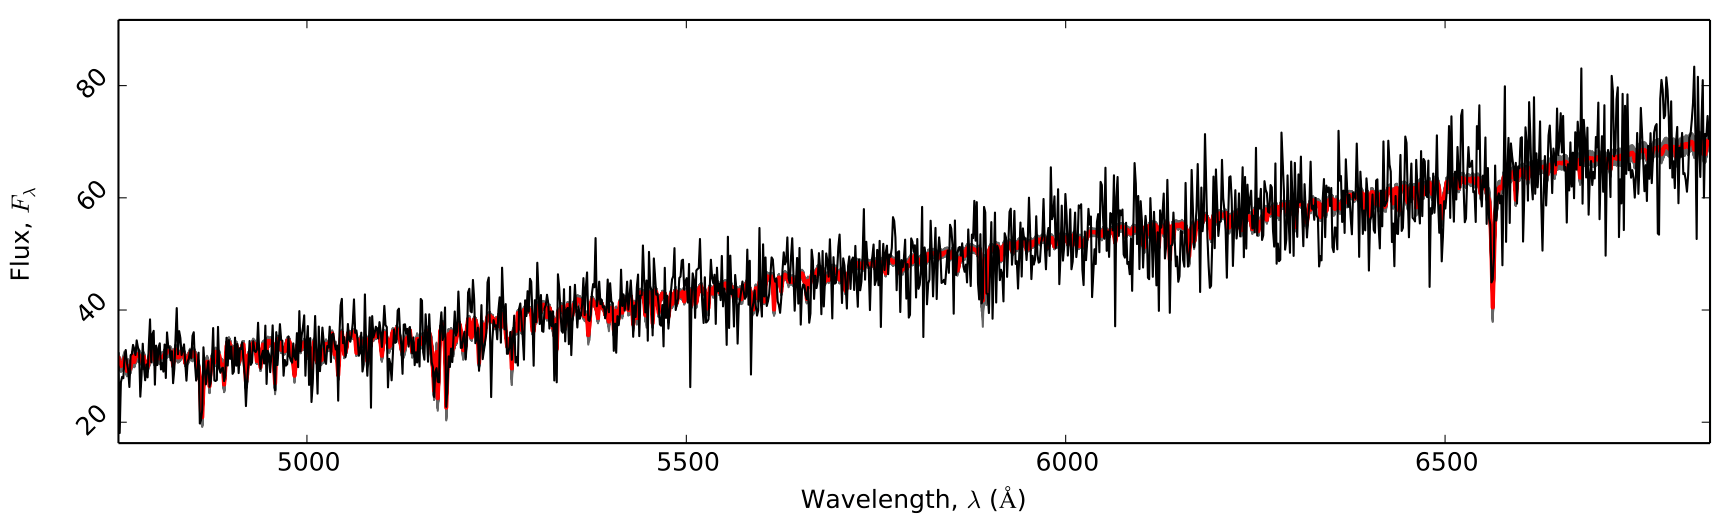
\includegraphics[width=\textwidth]{spectrum.pdf}
\caption{A faux observed spectrum (black) of $\mathcal{R} \sim 10000$ and S/N 
ratio of $\sim7$ with an underestimated variance by $\sim$10\% which was used for 
the self-consistent inference test. The recovered maximum likelihood model spectrum 
is shown in red. }
\end{figure*}


Default priors and configurations were employed. 200 walkers were used to explore 
the parameter space for 1250 steps as burn-in, and another 250 steps were used to 
sample the posterior. The chains for each parameter are shown in Figure 
\ref{fig:chains}. At least by eye, the chains appears to have converged after 
just 300 steps. The marginalised posterior distributions are shown in Figure 
\ref{fig:corner-inference}, with the accepted truth values marked. The true and 
inferred values for all parameters are tabulated in Table \ref{tab:inference-test}. 

This test demonstrates that accurate and precise inference of stellar parameters 
can be made even in the presence of substantial noise. The true values of all 
parameters are recovered within the uncertainties, and the largest (relative) 
uncertainties are observed for continuum coefficients $b_1$ and $b_2$. Figure 
\ref{fig:corner-inference} shows there are strong covariances between these 
parameters. This is unsurprising given the shape of the spectrum (Figure 
\ref{fig:spectrum-inference}), which could reasonably be fit with a linear 
continuum, even though the continuum was truly represented by a third order 
polynomial. The logarithm of additional fractional variance $\ln{f_{blue}}$ is 
precisely constrained, suggesting the noise model is excellently matched by the 
data. Given the simplicity of the noise model, the precision of inference on 
$\ln{f_{blue}}$ is unlikely to be recovered for real data.

\section{Utility}
\label{sec:examples}
Here I include two realistic applications to demonstrate the capabilities and 
ease-of-use of the software.
 
\subsection{Sol}
\label{sec:sun}
A high-resolution ($\mathcal{R} \sim$ 20000), high S/N ($\sim{}$150 pixel$^{-1}$) 
twilight spectrum was obtained from the GIRAFFE/FLAMES 
archive\footnote{eso.org/observing/dfo/quality/GIRAFFE/pipeline/solar.html}. 
The H875.7 setup was chosen for this example, yielding spectra from 848.2\,nm to 
899.2\,nm. Data points redder than 874\,nm have been discarded to more closely 
match the Gaia RVS wavelength coverage, and demonstrate the recoverability of 
stellar parameters on real data.

The AMBRE \citep{ambre} synthetic grid was also employed for this example. The 
continuum was represented with a third order polynomial, and no redshift or 
outlier modelling was included. The central $\pm$0.1 nm cores of the Ca II 
near-infrared triplet lines were masked (specifically rest wavelengths 
849.7-849.9\,nm, 854.1-854.3\,nm, and 866.1-866.3\,nm), as the cores are strongly 
affected by non-LTE effects that are not accounted for in the 1D LTE model atmospheres 
used to generate the AMBRE spectra. Pixels between rest wavelengths 850.10\,nm 
to 850.37\,nm were also masked as the models did not seem to accurately reproduce 
the data in this region. 

\begin{figure*}
\label{fig:solar}
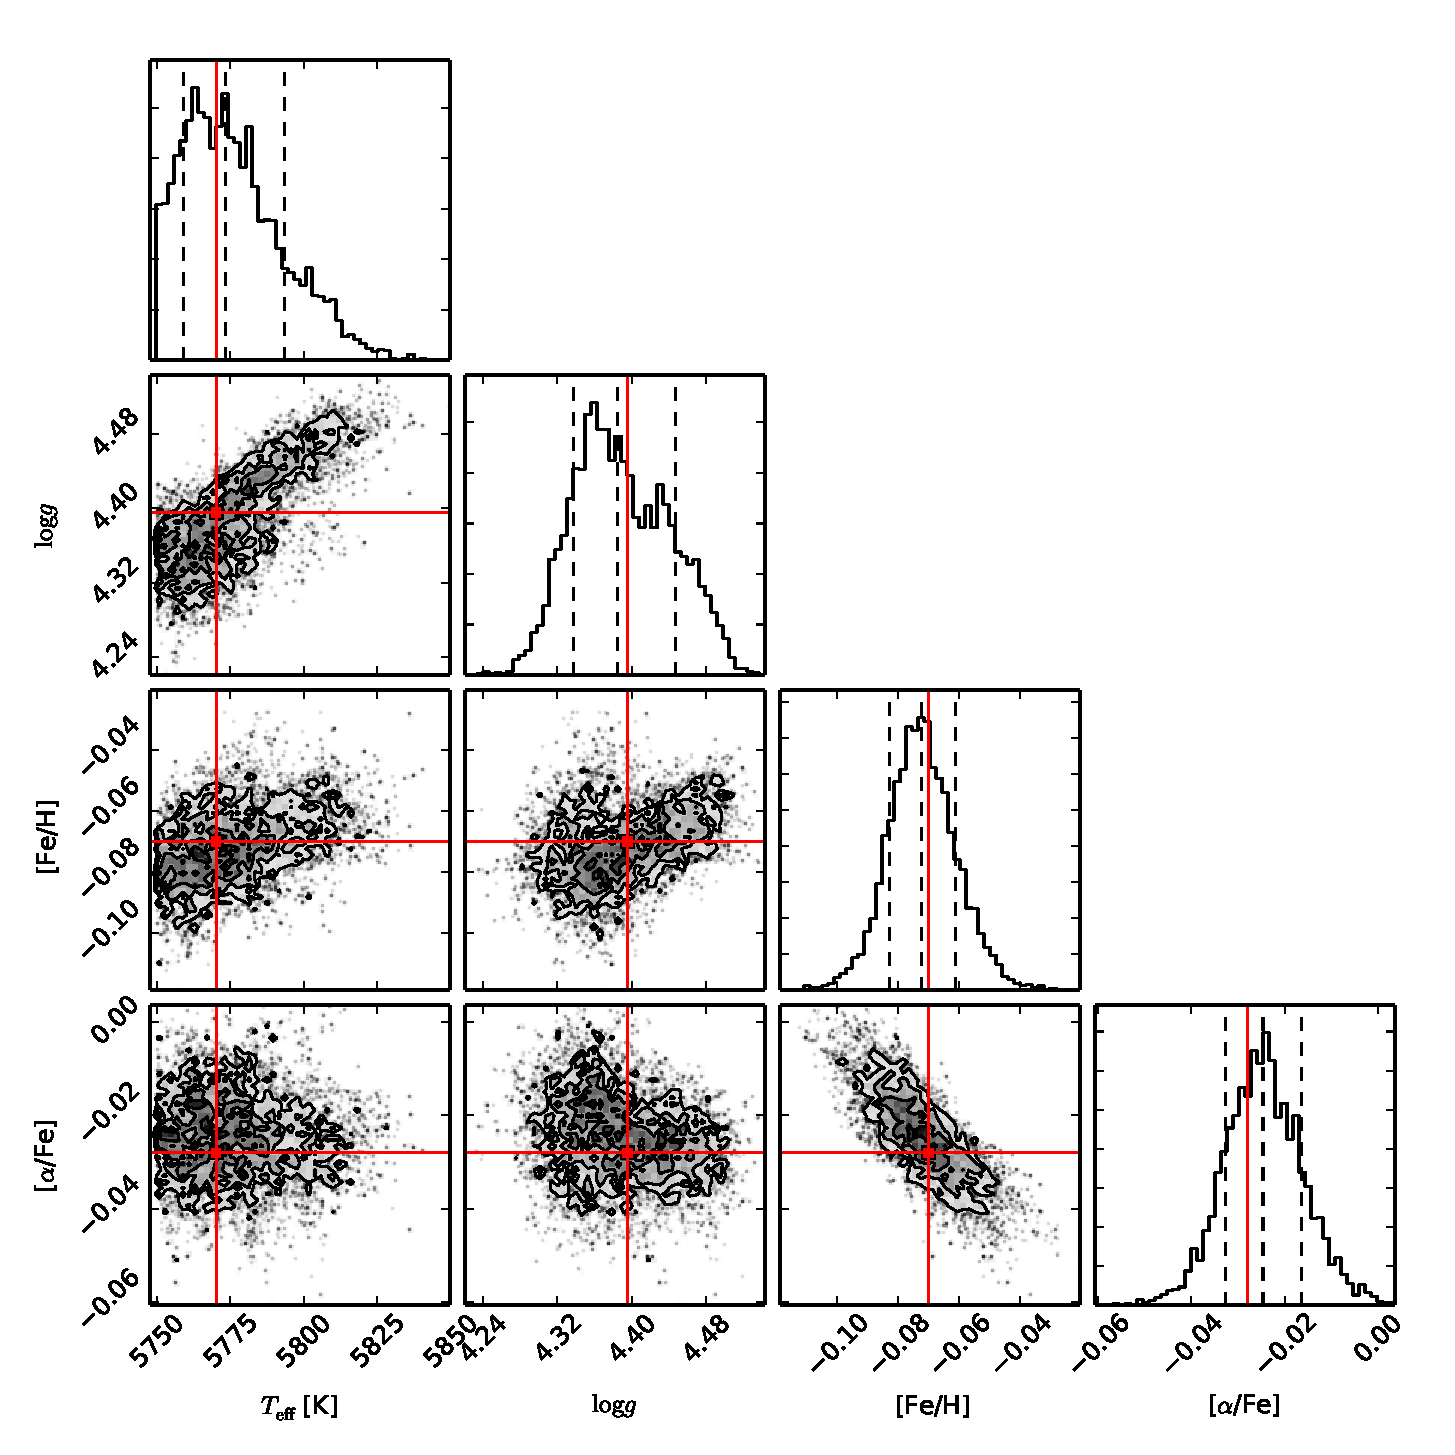
\includegraphics[width=\textwidth,height=\textwidth]{solar.pdf}
\caption{Stellar parameter ($\bm{\psi}$: $T_{\rm eff}$, $\log{g}$, [Fe/H], 
[$\alpha$/Fe])  posterior distributions for the GIRAFFE/FLAMES twilight spectrum. 
Nuisance parameters are not shown. Maximum likelihood values for each parameter 
are drawn in red, and the 16\%, 50\% and 84\% quantiles are shown as dashed lines. 
The posterior distributions are precise, and close to the accepted values (not 
shown) of $T_{\rm eff} = 5777$\,K, $\log{g} = 4.445$, slightly discrepant from 
[$\alpha$/Fe] = 0, and significantly deviant from [Fe/H] = 0. This test 
illustrates the precision achievable using \sick, but highlights the need for 
accurate models.}
\end{figure*}

For this example 1000 draws were made during the random scattering stage, and 
optimisation was performed using the default options. One hundred walkers 
explored the parameter space for 1000 steps, before another 200 steps were used 
to sample the posterior. The posterior distributions for stellar parameters is 
shown in Figure \ref{fig:solar}. The currently accepted stellar parameters for 
the Sun are $T_{\rm eff} = 5777$\,K, $\log{g} = 4.445$, [Fe/H] = 0, and 
[$\alpha$/Fe] = 0. The inferred parameters agree excellently with the accepted 
values for effective temperature and surface gravity: 
$T_{{\rm eff},inferred} = 5770^{+20}_{-14}$, and $\log{g}_{inferred} = 4.40^{+0.06}_{-0.05}$. 
The agreement is less pleasing for $\alpha$-element enhancement, and worse for 
mean metallicity: [$\alpha$/Fe]$_{inferred} = -0.03^{+0.01}_{-0.01}$, and 
[Fe/H]$_{inferred} = -0.07^{+0.01}_{-0.01}$. 

While our inferences are precise, the offset in mean metallicity suggest the 
models may be slightly inaccurate in this wavelength regime, or the solar abundances
employed are slightly discrepant, or perhaps there are 
unaccounted telluric features in the data. This test highlights the need to 
verify the accuracy of the input models. A useful extension of this project 
would be to simultaneously include telluric spectra, as well as pre-computed 
astereoseismic models, such that spectroscopy and time-series photometry could 
simultaneously constrain stellar parameters. Asteroseismology can accurately and 
precisely constrain surface gravity, but requires an input effective temperature. 
Conversely surface gravity is the least constrained stellar parameter by spectroscopy, 
but can precisely constrain effective temperature, and is the only method available 
to measure chemical abundances. Since \sick{} allows for any dispersion unit 
equivalency (e.g., frequency, wavelength, et cetera), spectroscopic and astereoseismic 
models can be trivially coupled into a generative framework for unprecedented 
accuracy and precision in stellar spectroscopy.

\subsection{Globular Clusters}
Globular cluster stars are excellent candidates for testing \sick{} over a large 
range of model parameters. Here I consider a realistic scenario of 
low-resolution, noisy spectra of red giant and asymptotic branch cluster 
candidates observed using the AAOmega spectrograph on the Anglo-Australian 
Telescope in Coonabarabran, Australia. The 580V and 1700D gratings were employed, 
yielding one channel between 370\,nm to 580\,nm with a spectral resolution 
$\mathcal{R} \sim 1300$, and another from 820\,nm to 890\,nm with spectral 
resolution $\mathcal{R} \sim 8000$.

Although these data are generally considered to be of low spectral resolution, 
I show that astrophysical parameters can be accurately inferred with high 
precision. The AMBRE synthetic grid has also been employed for this example. 
Each observed channel was treated identically: individual doppler shifts were 
permitted in each channel, and the continuum was represented as a second-order 
polynomial. Outlier modelling was included.
The parameter space was randomly sampled 1000 times before numerical optimisation 
was performed using the Nelder-Mead algorithm. 200 walkers explored the parameter 
space for a burn-in period of 450 steps, before sampling the posterior another 
50 times. The auto-correlation times, sampled chain values, and mean acceptance 
fractions demonstrated that convergence was unambiguously achieved for all 
analysed sources.

Radial velocities were used to identify and discard non-cluster members. The 
metallicity distribution of the remaining cluster stars are shown in Figure 
\ref{fig:clusters}, where a comparison to the literature is made. The 
\citet{harris} catalogue (accessed June 2014) has been used as a literature 
reference for all globular clusters. Note that although there are measurable 
intrinsic metallicity spreads and active debates on the mean abundances 
of these clusters, I have not adopted abscissa uncertainties.

\begin{figure}[h!]
\label{fig:clusters}
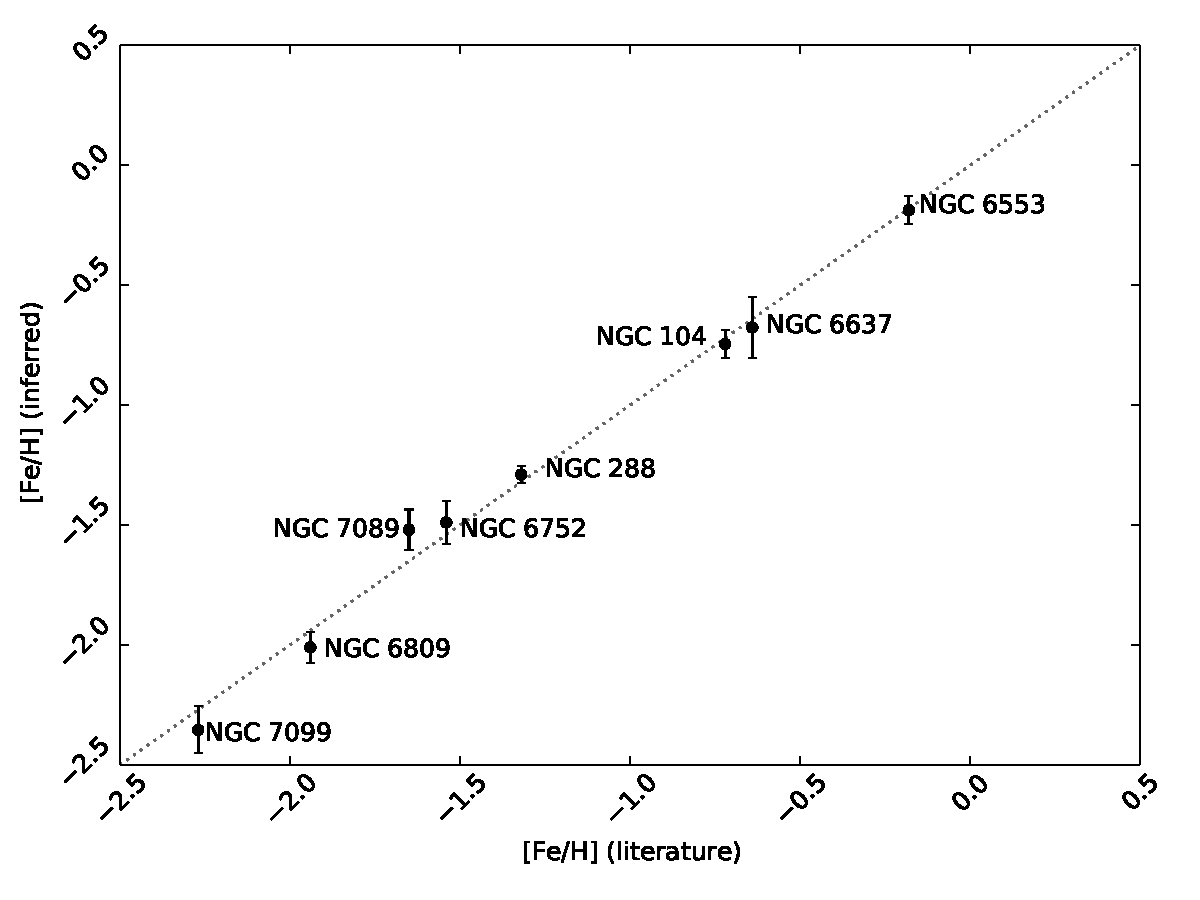
\includegraphics[width=0.5\textwidth]{clusters.pdf}
\caption{Metallicities of cluster stars inferred from noisy, low-resolution 
spectra obtained with the AAOmega spectrograph. The agreement with the 
literature values (see text) is very reasonable.}
\end{figure}

Even ignoring uncertainties in the literature values, the agreement between is 
exceptional for noisy, low-resolution spectra. No systematic trend is present 
and a negligible mean metallicity difference of $-0.001$ dex (an accuracy of $<$0.2\%) 
is observed over three orders of magnitude. The agreement would be remarkable 
for high-resolution spectra with exquisite S/N ratios. I emphasise that these 
results were obtained without performing any `calibration' or ad-hoc posterior 
corrections, which are usually entirely empirical and not motivated by an 
astrophysical understanding.

Individual uncertainties in stellar parameters are also extremely reasonable, 
particularly given the low spectral resolution and S/N of the data. Uncertainties 
of $\sim$75 K in $T_{\rm eff}$, $\sim$0.2 in $\log{g}$, $\sim$0.1 dex in [Fe/H] 
and $\sim$0.05 dex in [$\alpha$/Fe] are obtained in the presence of substantial 
noise (e.g., $S/N \sim 15$). The most uncertain results were obtained for 
{NGC\,7089}, where the lowest S/N ratios were achieved and only six cluster members were 
observed.

\section{Conclusion}
\label{sec:conclusions}

A probabilistic code has been introduced to approximately forward model 
spectroscopic data, and thereby allow for simultaneous inference of astrophysical 
and nuisance parameters. The generative model approach described here has a number 
of advantages over previously published techniques. Preparatory and subjective 
decisions (e.g., redshift and placement of continuum) are objectively treated 
within a scalar-justified mathematical model. This allows users to credibly 
characterise the parameter posterior distributions and understand how they affect 
astrophysical measurements. Until now most (if not all) published techniques treat 
these processes separately, thereby systematically biasing and generally 
under-estimating the parameter uncertainties.

With applications to both high- and low-resolution stellar spectra, I have 
demonstrated that the simultaneous incorporation of these effects leads to 
remarkable improvements in both accuracy and precision. While the examples 
presented here have focussed on stellar spectra, the code is ambivalent about 
\textit{what} the astrophysical parameters describe: the framework can be easily 
used for any kind of quantifiable astrophysical process. The code is MIT-licensed 
(freely distributable, open source) and has an extensive automatic testing suite, 
which includes regular reproduction of the examples presented in this \article{}. 
Complete documentation is available online\footnote{astrowizici.st/sick}, 
which includes a number of additional examples and tutorials. In the spirit of 
full scientific reproducibility, the online documentation is complemented with the 
files necessary to reproduce all of the examples presented in this \article{}. 
The source code is distributed using \textsc{git}, and hosted online at 
GitHub\footnote{github.com/andycasey/sick}. 

Great care has been spent to ensure the code is easy to use, and allow users to 
obtain precise inferences with little effort. I strongly encourage the use of this 
software for existing and future spectral datasets. With the sheer volume and 
high-quality of spectral data available, astronomers must begin to adopt objective, 
generative models for their data. Subtle astrophysical processes can only be 
discovered and understood with the proper characterisation of uncertainties 
afforded by generative models.

\acknowledgements
I am pleased to thank Louise Howes for extensive testing of this code, Martin 
Asplund for providing commentary, as well as Sergey Koposov and Jarryd Page for 
constructive discussions on this work. This research has made extensive use of NASA's 
Astrophysics Data System Bibliographic Services, the Coveralls continuous 
integration service, GitHub, and the \textsc{triangle.py} code \citep{triangle.py}.
This research has been funded by European Research Council grant 320360: 
The Gaia-ESO Milky Way Survey. 


\bibliographystyle{apj}
\bibliography{biblio}
\end{document}
